\label{ch:method}

For further details on MOAA's workflow, refer to \cite{fairhurst_MOAA_2023}.

% On the capsule design - \cite{HFIR}
The experiment design utilized in this work is based on the standard finned rabbit utilized in HFIR for isotope production.
The model neglects the fins for simplicity.

The term rabbit housing refers to the outer capsule (typically aluminum) used to contain the sample material.
The rabbit housing is in direct contact with the reactor primary coolant.
5 rabbit housing designs are hermetically sealed by welding and prevent direct contact of the enclosed sample material with the reactor coolant.
The rabbit consists of 3 pieces – a finned housing tube fabricated from extruded 6061-T6 aluminum and two 6061-T6 aluminum end plugs that are welded to the housing tube.
The rabbit is used primarily to conduct irradiations in support of isotope production.




% How everything connects to each other ?? I think the titles are self-explanatories.
% This chapter describes the different methods implemented in this work.
% This chapter describes all the methods utilized in the calculations.
% All the utilized machine learning algorithms are explainde in this Chapter.
% Chapter 5 explains their implentation in our work.

\section{Computational Tools}

% missing something here
% General description of each tool
% Let's go from lower to larger level of complexity

\subsection{MCNP}

% fairhurst-agosta_demonstration_2022
MCNP is a general-purpose, continuous-energy, generalized-geometry, Monte Carlo radiation-transport tool that can track neutrons, photons, electrons, and other particles.
It is developed and maintained by the \gls*{LANL} and was first released in 1983.

Monte Carlo calculations simulate the life of particles from their emission until their eventual absorption or escape of the system boundaries \cite{leppanen_devel_2007}, randomly sampling the frequency of the various interactions that the particles may undergo.
% The frequency and outcome of the various interactions that may occur during the particle’s life are randomly sampled and simulated according to interaction laws derived from particle physics.
The simulation of the particle interactions is repeated for a large number times, and the result is a detailed simulation of the transport process.

The main advantage of the Monte Carlo method is its capability to model geometry and interaction physics without significant approximations.
Some application areas of Monte Carlo neutron transport include reactor physics, nuclear criticality safety, radiation shielding and dosimetry, detector design and analysis, and fission and fusion reactor design.

The \gls*{MOAA} tool (Section \ref{sec:MOAA}) relies on MCNP for obtaining the geometry and material dependent parameters of the user-defined system during the experiment irradiation.
Additionally, MCNP runs photon-transport simulations to determine the energy deposition in the experiment.
This work uses version 6.2 of MCNP.


\subsection{ORIGEN/SCALE}

% fairhurst-agosta_decay_2022
ORIGEN is a general-purpose point depletion and decay tool to calculate isotopic concentrations, radiation source terms, and decay heat.
It is developed and maintained by the \gls*{ORNL}, and it has been available to regulators, licensees, and research institutions since 1980.

% fairhurst-agosta_demonstration_2022 (long version actually)
ORIGEN computes the time-dependent concentrations and source terms of a large number of isotopes subject to irradiation or decay.
The calculation considers the isotopic generation and depletion by neutronic transmutation, fission, radioactive decay, and physical or chemical feed and removal.
Some of its common applications are fuel irradiation calculations within nuclear reactors and spent nuclear fuel characterization for management, transportation, or storage.
Several of its capabilities include the estimation of isotope activities, radiotoxicity, decay heat, and emission rates for neutron and gamma particles.

ORIGEN is integrated into the SCALE Code System, which is a modeling and simulation suite for nuclear safety analysis and design \cite{scale}.
% COUPLE and OPUS
Besides ORIGEN, this work uses other modules of SCALE as well: COUPLE and OPUS.
ORIGEN requires a single space and spectrum-weighted cross-section library, that the user can generate using COUPLE.
The OPUS module provides the ability to extract specific data from the ORIGEN output libraries, perform unit conversions, and generate data for post-calculation analysis.
This work uses version 6.2.4 of SCALE.


\subsection{MOAA}
\label{sec:MOAA}

% What is MOAA? fairhurst-agosta_decay_2022 & fairhurst-agosta_development_2022
The Irradiation Experiment Neutronics Analysis group at the \gls*{INL} supports the \gls*{ATR} and \gls*{TREAT} by carrying out neutronics analyses before the irradiation of experiments takes place.
The analyses provide the radioisotope source term of the experiments after irradiation.
The calculated source terms have multiple applications, including inventory and shipping purposes, demonstration of compliance with the safety limits, comparison to \gls*{PIE} results, etc.

The Irradiation Experiment Neutronics Analysis group developed the MOAA tool, or just MOAA, to streamline the calculation of the experiment source terms \cite{fairhurst-agosta_development_2022}.
Overall, MOAA calculates radionuclide activity, mass, heat, and prompt and delayed gamma source distributions.
MOAA couples MCNP and ORIGEN by writing MCNP tally cards, reading MCNP tallies, creating ORIGEN input files, executing SCALE, and standardizing the results post-processing.
Streamlining this procedure helps to reduce processing times and avoid potential human errors.

% MOAA's Workflow: fairhurst-agosta_development_2022
MOAA can handle material activation/irradiation and decay calculations, which can be classified into single- or multi-case.
While single-case calculations use a single MCNP input file and a constant power irradiation, multi-case calculations can handle multiple MCNP input files with several core configurations and piecewise constant power irradiations (i.e., different power levels at each time step). % or a power history
Such a capability allows for the modeling of changes in material density, temperature, and geometry, as well as the control rod movement during the irradiation cycle.
For the sake of simplicity, the remainder of this section describes the single-case calculation scheme.

% Formulas
MOAA estimates the neutron flux, spectrum, and microscopic one-group cross-sections in user-defined cells using the following formulas
\begin{align}
\phi_T &= \frac{\nu \times P [MW]}{Q [MeV/fiss] \times k_{eff} \times 1.6022 \times 10^{-19}} \times F4_{SD} \\
\phi_{unnorm, E} &= F4_E \\
\sigma_i &= \frac{ F4_{FMi, SD} }{ F4_{SD} } \\  % F4 tally_{FM, SD}: the reaction cross-sections are microscropic (MCNP manual 3.3.5.7 Note 4)
% i &= (n,\gamma), (n,p), (n,2n), (n,\alpha), (n,fission)
i &= (n,\gamma), (n,p), (n,\alpha), (n,fission)
\end{align}
where $\phi_T$ is the total flux, $\nu$ is the number of neutrons emitted per fission, $P$ is the reactor power, $Q$ is the released energy per fission, $k_{eff}$ is the effective multiplication factor, $F4_{SD}$ is the F4 tally divided by the cell volume, $\phi_{unnorm, E}$ is the unnormalized spectrum, $F4_E$ is the F4 tally split up into energy bins, $\sigma_i$ is the microscopic cross-sections for reaction type $i$, and $F4_{FMi, SD}$ is the F4 tally for reaction type $i$ divided by the cell volume.
MOAA extracts the parameters $\nu$, $k_{eff}$, $F4_{SD}$, $F4_E$, and $F4_{FMi, SD}$ from the MCNP results, and $P$ and $Q$ are user-defined parameters.

Figure \ref{fig:moaa-workflow} provides a graphical representation of MOAA's workflow.
The MCNP transport simulation is based on ENDF/B-VII.1 nuclear data.
MOAA feeds $\phi_{unnorm, E}$ to COUPLE for calculating spectrum-weighted cross-sections using JEFF-3.0/A-based multigroup cross-sections.
Furthermore, MOAA provides COUPLE with $\sigma_i$ to replace the spectrum-weighted cross-sections.
% This final step means that the generated cross-section library is specific to the input model.
ORIGEN conducts the depletion calculations based on the COUPLE cross-section library.
Finally, MOAA uses OPUS to extract from the ORIGEN output libraries the data of interest, i.e., total decay heat ($H_L$), total gamma heating ($H_{\gamma,L}$), and the photon source energy distribution ($\varphi^{\gamma}$).

% Note: coupling between MCNP and ORIGEN flows in one direction.
% The assumption used for this method was that the depletion of the target would not impact the flux spectrum of the system sufficiently to require an iterative depletion calculation.


% ORIGEN decay and fission yield data come from ENDF/B-VII.1 and ENDF/B-VII.0, respectively.

% Section 5.2.3 Neutron Reaction Resource of \cite{scale}
% The JEFF-3.0/A files contain continuous energy neutron data for 774 target nuclei, including ground and metastable excited states, and 12,617 neutron-induced reactions below 20 MeV.
% Neutron reactions are available for 23 reaction types, including (n,n′), (n,2n), (n,3n), (n,f), (n,n′α), (n,2nα), (n,3nα), (n,n′p), (n,n2α), (n,n′d), (n,n′t), (n,n′ $3^$He), (n,4n), (n,2np), (n,γ), (n,p), (n,d), (n,t), (n, $3^$He), (n,α), (n,2α), (n,2p), and (n,pα).
% Implementation of the JEFF-3.0/A cross sections as ORIGEN multigroup data was accomplished by processing and collapsing the JEFF-3.0/A pointwise cross sections into a standard multigroup AMPX format using ENDF data-processing modules of the AMPX 7 cross section processing code system.
% The collapse is performed using a thermal Maxwellian–1/E–fission–1/E weighting spectrum (see Figure 5.2.1) to provide infinite dilution multigroup cross sections.
% Cross section data from the JEFF-3.0/A neutron activation file are first converted to point-wise cross section data, are Doppler broadened to 900K, and then they are collapsed to different group structures.
% The following group strucures are available in SCALE: ..., 252-group neutron (thermal applications), ...
% Before the cross sections in ORIGEN can be used, they must be collapsed with a user-defined multigroup flux to a one-group cross section and added to the ORIGEN binary library (see the COUPLE input description).

% According to the 6.2.4 manual, ORIGEN uses JEFF-3.0/A
% But according to SCALE 6.2 ORIGEN Training Course Oak Ridge National Laboratory March 1–4, 2021, ORIGEN uses JEFF-3.1/A.
% I believe, SCALE in Sawtooth is using data from SCALE 6.2.3, so I think I am using JEFF-3.0/A actually.

% Sublet, et al. The JEFF-3.0/A Neutron Activation File—New Features, Validation, and Usage. 2005.
% https://aip.scitation.org/doi/abs/10.1063/1.1944990
% 12,617 reactions total, breakdown by reaction type in Table 1.

\begin{figure}[htbp!] %htbp! or H
  \centering
  \includegraphics[width=0.75\linewidth]{figures/moaa-flow}
  \caption{Graphical representation of MOAA's workflow.}
  \label{fig:moaa-workflow}
\end{figure}


The code structure of MOAA comprises three python scripts: (1) \texttt{MOAA\_create\_tally}, (2) \texttt{MOAA\_create\_origen}, and (3) \texttt{MOAA\_combine\_results} \cite{fairhurst-agosta_development_2022}.
The routine usage of MOAA requires the successive run of these three scripts.
The calculations rely on pre-existing MCNP input files that define the experiment configuration, meaning that the user needs to create them before running MOAA.
The user specifies the calculation parameters of MOAA in a \texttt{YAML} file, including the MCNP cells that the user wants MOAA to run the calculations on.
For instance, if there is an experiment taking place in a small section of a reactor, the user might want to focus only on the cells defining the experiment, thereby becoming the cells of interest for MOAA.

\texttt{MOAA\_create\_tally} adds tallies to the MCNP input file.
Given the user-specified \texttt{YAML}, MOAA defines a total neutron flux tally, a neutron flux energy tally, and a reaction rate tally for the cells of interest.
The following step requires running MCNP externally.
Although the execution of MCNP does not happen automatically, it is a necessary step in the calculations and the reason for including it in this description.

\texttt{MOAA\_create\_origen} uses the MCNP tally information for creating COUPLE, ORIGEN, and OPUS input sequences, executing SCALE, and handling the results.
MOAA reads the MCNP output file containing the energy and the reaction rate tallies to define the COUPLE input sequence.
MOAA reads the MCNP input file to determine the material composition and densities of the cells of interest.
This information, along with the total flux tally and several user-defined parameters, allows MOAA to define the ORIGEN and OPUS input sequences.
The COUPLE, ORIGEN, and OPUS input sequences integrate the SCALE input files, and once generated, MOAA executes them.
Both the generation of the input files, as well as their execution, happen in parallel.
MOAA relies on the python standard library \texttt{asyncio}, which is the foundation for python asynchronous frameworks, allowing for the creation and execution of co-routines.
This feature allows for an overall reduction in the run times.
The final stage of this step is the handling of SCALE outputs.
The execution of SCALE produces \texttt{.plt} files, which MOAA translates into \texttt{.csv} format, facilitating post-processing of the results.

\texttt{MOAA\_combine\_results} combines the results for a set of user-defined cells of interest.
When several cells form a region of interest, this utility script combines the source term from all of them.
This utility is helpful in cases where an experiment capsule is defined by multiple cells and materials.
This step allows for computing a source term for the whole capsule, for example.


\subsection{Serpent}

The Serpent Monte Carlo code \cite{leppanen_serpent_2015} is a three-dimensional continuous-energy neutron transport application developed by the VTT Technical Research Centre of Finland, and it has been in public distribution since 2009.
This work uses Serpent 2.1.32 and the cross-section library ENDF/B-VII.0 for the calculations.
The choice of nuclear data was based on their availability.

In general, Serpent serves two purposes: (1) group constant generation and (2) reactor modeling.
In group constant generation, the transport simulation produces input parameters for a deterministic solver.
In reactor modeling, the Monte Carlo simulation itself represents the solution to the full-scale problem.

This work uses Serpent because of its built-in burnup calculation routine.
Moreover, Serpent is capable of calculating delayed gamma heating in a two-step process.
The first step consists of a transport/depletion calculation that saves the radioactive material composition in a binary restart file.
The second step is a photon-transport simulation that generates the photon source based on the binary restart file.
This second simulation creates a \textit{\_gsrc.m} file specifying the gamma source distribution (see Appendix \ref{ap:serpent_gsrc} for further details).
This work uses Serpent for a code-to-code comparison exercise against MOAA and the nuclear heating calculation module.


\subsection{OpenFOAM}

% fairhurst-agosta_machine_2_2022
OpenFOAM \cite{weller_tensorial_1998} is a \gls*{FVM} C++ class library originally released as the Field Operation And Manipulation (FOAM) library in 1989, becoming open-source in 2004.
Since its initial release, the core design of OpenFOAM has remained the same, comprising an extensible  range of libraries, solvers, and pre and post-processing tools.

The developers intended to make the top-level syntax of the code as close as possible to conventional mathematical notation.
The result is a C++ class library capable of modeling continuum-mechanics phenomena, including incompressible and compressible flow, multiphase flow, and various turbulence modeling techniques.
Although it primarily targets \gls*{CFD} problems, it solves other continuum-mechanics problems as well, such as structural mechanics \cite{weller_tensorial_1998} or molecular dynamics \cite{longshaw_mdfoam_2018}.
Moreover, it supports parallelization via domain decomposition, in which each available processor runs the code in each mesh subdomain.

This work uses OpenFOAM as the main thermal-fluids solver and calculates the capsule temperature during the channel draining event.
The calculations use OpenFOAM v2012 and the application \textit{chtMultiRegionFoam}.


\subsection{MOOSE}

% fairhurst-agosta_machine_2_2022
The \gls*{MOOSE} \cite{gaston_moose_2009}, originally released in 2008, is an open-source \gls*{FEM} framework that supports engineering analysis applications, targeting systems of non-linear partial differential equations.
The MOOSE applications define weak forms of the governing equations and modularize the physics expressions into \textit{kernels}.
The kernels are C++ classes containing methods for computing the residual and Jacobian contributions of individual pieces of the governing equations.
All the software built on the MOOSE framework shares the same \gls*{API}.
This feature facilitates a relatively easy coupling between different phenomena.
Additionally, the framework and its applications use \gls*{MPI} for parallel communication and allow deployment on massively-parallel cluster-computing platforms.

% MOOSE role in the calculations
In this work, MOOSE solves a simplified thermal-fluids model (Chapter \ref{ch:tf}) to examine the applicability of machine learning to capture the experiment thermal behavior.
Three reasons motivated the choice of MOOSE for such a study.
First, the author’s familiarity with the software made it the natural choice.
Second, the MOOSE input sequence consists of only one script, while OpenFOAM’s comprises several scripts.
Defining the input sequence with only one script reduces the burden of handling a large number of files.
Third, the MOOSE model uses the Boussinesq approximation to reduce the computational expense of the simulation.
The approximation considers that the density-variation effects are only present in the body force term of the conservation of momentum equations.
This approximation reduces the system of equations in the fluid region to three equations.

Nevertheless, further inspection of the thermal-fluids model revealed that even when MOOSE uses the Boussinesq approximation and OpenFOAM does not, OpenFOAM simulations are considerably faster.
This reason motivated the choice of OpenFOAM as the main solver for future studies.
Furthermore, OpenFOAM has several turbulence models readily available and is capable of solving the density, motion, and temperature of the air without approximations.


\section{Nuclear Heating Calculation}

% fairhurst-agosta_decay_2022 & fairhurst-agosta_demonstration_2022
% The following equations calculate the nuclear heat deposition in the experiment
% \begin{align}
% TH [W] &= Q_{T} - Q_{\gamma, T} + Q_{\gamma, L}  \label{eq-heat} \\
% Q_{\gamma, L} [W] &= 1.60217733 \times 10^{-13} \times \: ^* \! F8 [MeV] \times \mathlarger{\sum}_i S_i \\
% S_i[\gamma/s] &= \int_{E} \varphi^\gamma_i(E) dE
% \end{align}
% where $TH$ is the total heat deposited in the region of interest, $Q_T$ is the total decay heat, $Q_{\gamma, T}$ is the total gamma heating, $Q_{\gamma, L}$ is the energy deposited locally by the gamma radiation, $^\ast F8$ is the energy deposition $^\ast$F8 tally, $S_i$ is the total gamma emission rate for the region of interest $i$, and $\phi^\gamma_i(E)$ the photon source energy distribution.

The following equations calculate the deposition of the nuclear heat in the experiment
\begin{align}
H_{T} [W] &= H_{ch} + H_{\gamma, Tr}  \label{eq-heat} \\
H_{ch} [W] &= H_{T, L} - H_{\gamma, L} \\
H_{\gamma, Tr} [W] &= 1.6022 \times 10^{-13} \times \: ^* \! F8 [MeV] \times \mathlarger{\sum}_i S_i \\
S_i[\gamma/s] &= \int_{E} \varphi^\gamma_i(E) dE
\end{align}
where $H_{T}$ is the total heat deposited in the region of interest, $H_L$ is the total decay heat, $H_{\gamma, L}$ is the total gamma heating, $H_{\gamma, Tr}$ is the energy deposited in the region of interest resulting from the photon transport, $^\ast F8$ is the energy deposition calculated by an $^\ast$F8 tally, $S_i$ is the total gamma emission rate for the region of interest $i$, and $\phi^\gamma_i(E)$ the photon source energy distribution.

% Overall the calculation scheme follows the formal 3-step process, in which MOAA conducts the first two steps, and multiple MCNP photon-transport calculate the delayed gamma heating.
As shown in Figure \ref{fig:heat-flow}, the nuclear heating calculation relies primarily on \gls*{MOAA}.
ORIGEN calculates $H_L$ and $H_{\gamma, L}$ assuming those to be locally deposited.
An MCNP photon-transport simulation estimates $^\ast F8$, which allows to calculate $H_{\gamma, Tr}$.
MOAA provides the photon source energy distribution of the cells of interest which allow to define a fixed photon source in MCNP.
For further details on the algorithm implementation refer to Appendix \ref{ap:mcnp_fixed}.

\begin{figure}[htbp!] %htbp! or H
  \centering
  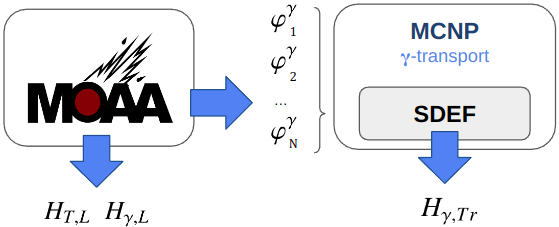
\includegraphics[width=0.8\linewidth]{figures/heat-flow}
  \caption{Nuclear heating calculation scheme.}
  \label{fig:heat-flow}
\end{figure}

% Maybe I should put the thermal-fluids model here ... not sure

\section{Generalization of the Nuclear Heating Calculation}
\label{sec:3-gen}

% % Nuclear Physics Theory - Maybe
% \input{nuclear_physics}

Up to this point, this document explained the scheme for estimating the nuclear heating for a certain experiment.
The database creation utilizes this calculation scheme repeatedly to obtain the nuclear heating for experiments composed of individual materials.
Nevertheless, an experiment usually comprises a mix of different materials.
Hence, this section establishes a method relying on the database to calculate the nuclear heating in the experiment for any given composition.

The method uses the nuclear heating of the individual components of the mix.

For example, if we wanted to calculate the nuclear heating in a stainless steel sample, and let it be composed of iron, carbon, chromium, and nickel, we would need to compute first the nuclear heating for those elements independently, and based on them, the heating of the mix.

For example, if we wanted to calculate the nuclear heating in a stainless steel sample, and let it be composed of iron, carbon, chromium, and nickel, we would need to compute first the nuclear heating for individual experiments of iron, carbon, chromium, and nickel first.
The method calculates the heating of the mix based on the individual calculations.
The following formula calculates the nuclear heating of a mix of different materials
\begin{align}
H_{j,M} &= \mathlarger{\sum}_i H_{j,i}(\rho_i)  \label{eq:data-1} \\
H_{j,i}(\rho_i) &= \rho_i f(\rho_i)  \label{eq:data-2} \\
f_{non-fiss}(\rho_i) &= H_{j,i}^o / \rho_i^o  \label{eq:data-3} \\
f_{fiss}(\rho_i) &= H_{j,i}^k(\rho_i^k) / \rho_i^k  \label{eq:data-4}
\end{align}
where $H_{j, M}$ is the heating component $j$ of the mix and $\rho$ is the density.
The heating component $j$ could be either the charged particles, transported gammas, or total contributions.
$H_{j,i}$ and $\rho_i$ correspond to the heating values and density of material $i$ in the mix.

The calculation contemplates two possible types of materials, fissile and non-fissile.
The calculation of $H_{j,i}(\rho_i)$ requires a functional form for $f(\rho_i)$, being constant for non-fissile (eq. \ref{eq:data-3}) and density-dependent for fissile materials (eq. \ref{eq:data-4}).
$H_{j,i}^o$ corresponds to the heating values for an experiment made of material $i$ only with a density value equal to its theoretical density $\rho_i^o$.
$H_{j,i}^k$ corresponds to the heating values for an experiment made of material $i$ only with a density value equal to $\rho_i^k$.
As $f_{fiss}$ is density-dependent, it requires a non-linear interpolation of several values of $H_{i,j}^k/\rho_i^k$.
Chapter \ref{ch:neut} verifies this model by applying the methodology to experiments of different material compositions.


\section{Thermal-Fluids Calculations}
\label{ch3-tf}

% Model description
The thermal-fluids model calculates the evolution of the capsule temperature after reactor shutdown.
Figure \ref{fig:thermal-model} shows the simplified thermal-fluids model of an experiment.
The model comprises a conjugate heat transfer problem, characterized by a cavity filled with air and a multi-region solid.
The solid consists of an experiment embedded in a capsule.
This model represents a post-irradiation experimental device that is cooled by the natural circulation of air.
Note that the model is generic and reactor-agnostic, meaning that it can be tailored to any research reactor.
The final dimensions of the model are specific to each experiment.
% To decrease the computational burden, we reduced the model to a two-dimensional problem.

\begin{figure}[htbp!] %htbp! or H
  \centering
  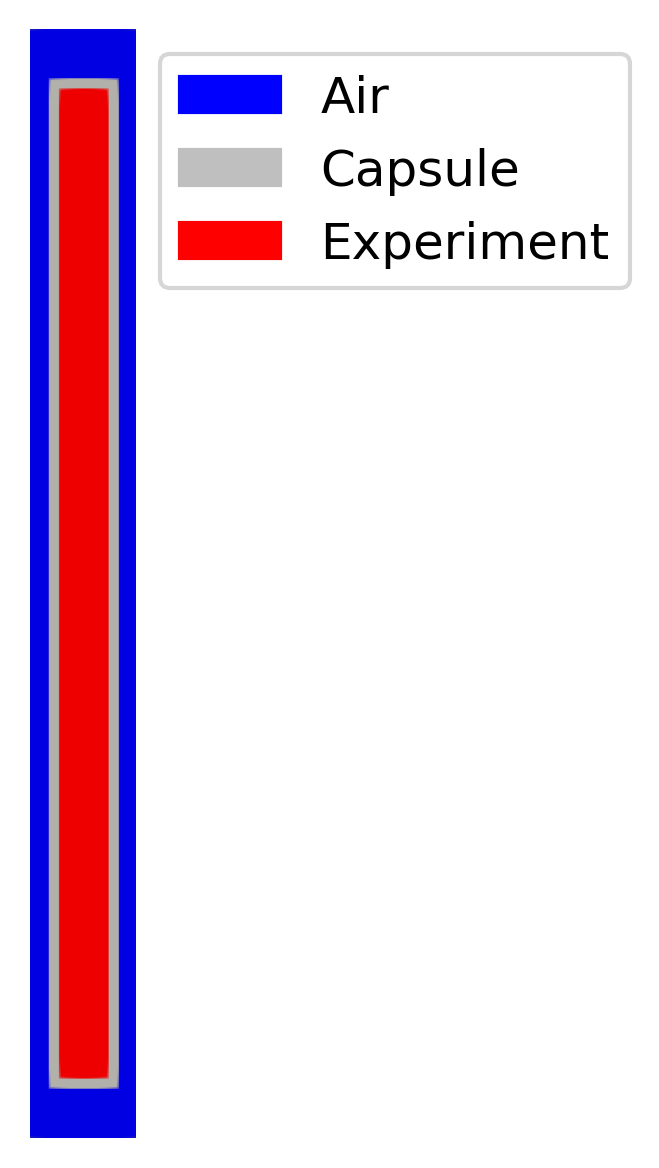
\includegraphics[width=0.2\linewidth]{figures/tf-geo}
  \caption{Thermal-fluids model of an experiment in an irradiation channel. Dimensions not at scale to better display the model regions.}
  \label{fig:thermal-model}
\end{figure}

Table \ref{tab:tf-mat} summarizes the model material properties.
The material properties of the capsule correspond to Aluminum 6061 T6.
Since the experiment material is variable, its material properties are not fixed and are not shown here.

\begin{table}[htbp!]
  \centering
  \caption{Material properties of the thermal-fluids model.}
  \label{tab:tf-mat}
  \begin{tabular}{cccc}
    \toprule
      Properties & Units & Air & Capsule \\
    \midrule
      $\rho$ & kg/m$^3$ & 1.2 & 2.7 $\times$ 10$^{3}$ \\
      $k$ & W/m/K & 2.6 $\times$ 10$^{-2}$ & 167 \\
      $c_p$ & J/kg/K & 1000 & 1256 \\
      $\mu$ & kg/m/s & 1.8 $\times$ 10$^{-5}$ & - \\
      $\beta$ & 1/K & 3.356 $\times$ 10$^{-3}$ & - \\
    \bottomrule
  \end{tabular}
\end{table}

% Equations: solve the air density
% https://caefn.com/openfoam/solvers-buoyantpimplefoam
% More equations:
% https://cfd.direct/openfoam/energy-equation/
% https://doc.cfd.direct/openfoam/user-guide-v6/thermophysical
% https://www.openfoam.com/documentation/guides/latest/api/hConstThermoI_8H_source.html
% https://github.com/OpenFOAM/OpenFOAM-dev/blob/master/src/thermophysicalModels/basic/rhoThermo/heRhoThermo.C
% https://www.cfd-online.com/Forums/openfoam-programming-development/222965-temperature-calculation-enthalpy.html
The mass, momentum, and energy conservation equations (\ref{eq:consv-mass}-\ref{eq:consv-ene-f}) along with the equation of state (\ref{eq:state}) allow to solve the motion and temperature of the air \cite{openfoam}, and the heat conduction equation (\ref{eq:consv-ene-s}) to solve the temperature in the solid regions:
\begin{align}
& \frac{\partial}{\partial t} \rho + \nabla \cdot (\rho \bar{u}) = 0  \label{eq:consv-mass} \\
& \left( \frac{\partial}{\partial t} (\rho \bar{u}) + \nabla \cdot \left( \rho \bar{u u} \right) \right) + \nabla p - \rho \bar{g} - \mu \Delta \bar{u} = 0 \label{eq:consv-mom} \\
& \left( \frac{\partial}{\partial t} (\rho h) + \nabla \cdot \left( \rho \bar{u} h \right) \right) + \frac{\partial}{\partial t} \left( \rho \frac{|\bar{u}|^2}{2} \right) + \nabla \cdot \left( \rho \bar{u} \frac{|\bar{u}|^2}{2} \right) - \frac{\partial}{\partial t}p - \alpha \Delta h - \rho \bar{g} \cdot \bar{u} = 0 \label{eq:consv-ene-f} \\
& p = \rho R T \label{eq:state} \\
& h = c_p T \\
& \rho c_p \frac{\partial}{\partial t} T - k \Delta T - q''' = 0 \label{eq:consv-ene-s}
\end{align}
where $\rho$ is the density, $\bar{u}$ is the velocity, $p$ is the pressure, $\bar{g}$ is the gravity, $\mu$ is the dynamic viscosity, $h$ is the enthalpy, $\alpha$ is the thermal diffusivity, $R$ is the ideal gas constant, $c_p$ is the heat capacity, $T$ is the temperature, $k$ is the thermal conductivity, and $q'''$ is the volumetric heat source provided by the nuclear heat calculation module.

% Turbulence ?
% Radiation Heat Transfer ?

% As mentioned earlier, Chapter \ref{ch-tf} solves a simplified version of this thermal-fluids model using MOOSE.
% Future 


\section{Machine Learning}

% Classification
This work uses several classification algorithms to determine if the capsule encasing the experiment melts in case of a channel draining event.
Classification is the process of recognizing certain patterns in a dataset, and grouping the samples into categories based on those patterns.
Machine learning classification algorithms use input training data to determine such categories and then predict the likelihood that subsequent data points will fall into them.
This work utilizes the following classification techniques: \Gls*{SVM}, \Gls*{DT}, \Gls*{RF}, \Gls*{KNN}, \Gls*{LogR}, and \Glspl*{FNN}.

% Regression
Additionally, this work utilizes several methods to predict the time evolution of the capsule temperature.
These methods rely on the following algorithms: \Gls*{DTR}, \Gls*{RFR}, \Glspl*{FNN}, and \Glspl*{LSTM}.
% Packages
The implementation of the FNNs and LSTMs utilizes \textit{Keras} \cite{chollet_keras_2015} and the rest of the models
utilize \textit{scikit-learn} \cite{pedregosa_scikit-learn_2011}.
This section presents a brief introduction to the different machine learning algorithms.
Chapter \ref{ch:tf} describes in detail the data preparation process.


\subsection{Support Vector Machine}

% https://scikit-learn.org/stable/modules/svm.html#mathematical-formulation
% see http://web.mit.edu/6.034/wwwbob/svm-notes-long-08.pdf
% bae_calculation_2008
% fletcher_support_2008

This algorithm searches for a hyperplane that separates the dataset.
The support vectors are a small subset of the training samples that are closest to this hyperplane.
The method determines the hyperplane that maximizes the distance or margin to the support vectors \cite{pedregosa_scikit-learn_2011}.

Equation \ref{eq-svm-1} defines the hyperplane, and equation \ref{eq-svm-2} the hyperplanes of the support vectors, where $\phi(x)$ is the transformation from feature to kernel space, to allow for non-linear solutions.
The margin between hyperplanes is equal to $1/||w||$, and then maximizing the margin is equivalent to minimizing $||w||$.
The optimization problem is solved by minimizing $J(w)$ in equation \label{eq-svm-3}
\begin{align}
&w \cdot \phi(x_i) + b = 0    \label{eq-svm-1} \\
&w \cdot \phi(x_i) + b = \pm1 \label{eq-svm-2} \\
J(w) &= \frac{1}{2} ||w||^2 + C \sum_i \xi_i \label{eq-svm-3} \\
\intertext{such that}
y_i(&w \cdot \phi(x_i) + b) \geq 1-\xi_i \\
& \xi_i \geq 0
\end{align}
where $C$ is the regularization factor, which gives more weight to minimizing the flatness or the error, $\xi_i$ is the slack variable, which guards against outliers.
Some problems are not perfectly separable with a hyperplane.
Equation \ref{eq-svm-3} allows some samples to be at a $\xi_i$ distance from their correct boundary.
A larger regularization parameter penalizes the approximation error, leading to its decrease during the optimization.
% An increase in the regularization parameter leads to a decrease of the approximation error.
% A larger $\epsilon$ decreases the number of support vectors, reducing the accuracy of the approximation.


\subsection{Decision Tree}

% steorts_tree_2017-1
% https://scikit-learn.org/stable/modules/tree.html#mathematical-formulation

The algorithm divides the predictor space into simple regions.
The set of splitting rules segmenting the predictor space can be visualized as an inverted tree.
Its branches connect internal nodes where a test determines in which sub-branch to continue.
The end of the tree contains the leaf nodes which make the final predictions.
The leaf nodes assign to new observations falling into those regions the most commonly occurring class of the training observations.

\Gls*{DT} uses a recursive binary split to grow the tree by minimizing an impurity function, which in this case is the Gini index \cite{pedregosa_scikit-learn_2011}, defined as
\begin{align}
& G = \sum_k p_{mk}(1-p_{mk}) \label{eq-dt}
\end{align}
where $p_{mk}$ is the proportion of class $k$ observations in the region node $m$.
A low Gini index indicates that a node contains predominantly observations from a single class.
Other measures of impurity include the entropy and the misclassification.
The package \textit{scikit-learn} uses the Gini index by default.

%The advantages of \glspl{DT} are that they are easy to interpret and that require little data preparation.
%Their main disadvantage is that complex trees are prone to overfitting.
%Predictions of decision trees are not continuous, but piecewise constant approximations.
%Therefore, they are not good at extrapolation.

% DTR
The algorithm for \gls*{DTR} is slightly different.
The tree can be visualized as a piecewise constant approximation.
For every new observation falling into the same space subregion, the leaf nodes assign the same prediction value, which is the average value of the training observations.
The training algorithm minimizes the \gls*{MSE} \cite{pedregosa_scikit-learn_2011}
\begin{align}
& MSE = \frac{1}{n_m} \sum_{y \in Q_m} \left( y - \bar{y}_m \right)^2 \label{eq-dtr} \\
& \bar{y}_m = \frac{1}{n_m} \sum_{y \in Q_m} y
\end{align}
where $\bar{y}_m$ is the learned mean value of the node.
$Q_m$ represents the data at node $m$ with $n_m$ samples.


\subsection{Random Forest}

% pedregosa_scikit-learn_2011

Individual DTs may exhibit high variance.
This method improves the performance of a single tree, by reducing the overfitting and increasing its precision.

The algorithm consists of a collection of decision trees.
It is based on the bootstrap aggregating method or \textit{bagging} \cite{breiman_bagging_1996}, which chooses the training data for each decision tree at random with replacement, fits the \glspl*{DT}, and then combines their results by voting.
The purpose of the randomness is to decrease the variance of the forest and decouple the prediction error \cite{pedregosa_scikit-learn_2011}.

% RFR
The algorithm for \gls*{RFR} is very similar, but instead of combining the different DT results by voting, the result is an average of the predictions of the different trees.


\subsection{K-Nearest Neighbors}

% https://scikit-learn.org/stable/modules/neighbors.html#classification

Neighbors-based classification does not create a model, but instead it stores instances of the training data \cite{pedregosa_scikit-learn_2011}.
Then, the algorithm classifies new samples based on the stored instances.
The KNNs are the $K$ training observations closest in distance to a new observation.
The Euclidean distance is the most common choice for measuring the distance between observations.
When classifying a new observation, the method assigns the data class which has the most representatives within the nearest neighbors of the point.
\gls*{KNN} is often successful in classification situations where the decision boundary is very irregular.


\subsection{Logistic Regression}

% https://scikit-learn.org/stable/modules/linear_model.html#logistic-regression

This type of regression determines the relationship between a binary dependent variable and a set of independent variables.
The method utilizes the sigmoid function, shown in equation \ref{eq:logR-1}, to determine the likelihood of an observation to fall within each category.
The method determines the coefficients of the sigmoid function by minimizing a certain cost function.
This work uses the default setting of \textit{scikit-learn} which is to minimize the $L_2$-penalized cost function $J(w)$
% What loss? also, L2 regularization
\begin{align}
& \sigma(x_i) = \frac{1}{1+e^{-(w \cdot x_i + b)}} \label{eq:logR-1} \\
& J(w) = \frac{1}{2} ||w||^2 + C \sum_i log(exp(-y_i(w \cdot x_i + b))+1) \label{eq:logR-2}
\end{align}
where $C$ is the regularization factor.
% Like in support vector machines, smaller values specify stronger regularization.
Like in SVM, a larger regularization factor decreases the approximation error during the optimization.


\subsection{Feed-forward Neural Networks}

\Glspl*{FNN} are deep-learning architectures that learn complex relationships between inputs and outputs by mimicking biological networks of neurons.
A network consists of an input and output layer, and $N$ hidden layers of neurons, as shown in Figure \ref{fig:3-fnn}.

\begin{figure}[htbp!] % or H
  \centering
  \begin{subfigure}[b]{0.51\textwidth}
    \centering
    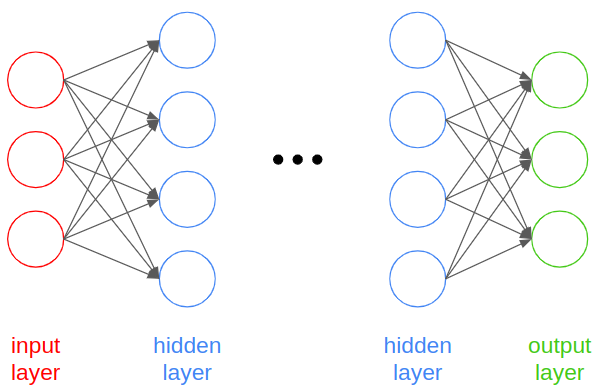
\includegraphics[width=1.0\textwidth]{figures/fnn-1}
    \caption{}
  \end{subfigure}
  \hfill
  \begin{subfigure}[b]{0.47\textwidth}
    \centering
    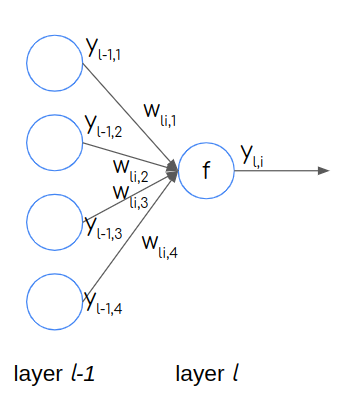
\includegraphics[width=0.65\textwidth]{figures/fnn-2}
    \caption{}
  \end{subfigure}
  \hfill
  \caption{Example of an FNN.}
  \label{fig:3-fnn}
\end{figure}

A neuron is connected to the neurons of the previous layer by weights.
Each neuron adds together the product of the neuron values in the previous layer and the weights connecting them plus a bias.
This summation serves as input to the next layer after applying an activation function, as stated in the following equation
\begin{align}
& y_{l, i} = f(w_{l, i}^T y_{l-1} + b_{l, i}) \label{eq-fnn-1} \\
& H = -\frac{1}{N} \sum_i y_i log(p(y_i)) + (1 - y_i) log(1 - p(y_i)) \label{eq-fnn-2}
\end{align}
where $y_{l, i}$ is the output of the node $i$ in layer $l$, $y_{l-1}$ output values of layer $l$-$1$, $f$ the activation function, and $w_{l, i}$ and $b_{l, i}$ the weights and biases connecting layer $l$-$1$ to the node $i$ of layer $l$.

Training the network sets the values of the connecting weights and biases by minimizing an error metric.
For the classification problem, the error metric is the binary cross-entropy, shown in equation \ref{eq-fnn-2}, where $y_i$ is the label, $p(y_i)$ is the predicted probability of the point to be \textit{true}, and $N$ is the number of samples.

% FNNs for regression
When using the FNN for regression, the algorithm trains the network by minimizing the MSE
\begin{align}
MSE = \frac{1}{N} \sum_i (Y_i - \hat{Y_i})^2 \label{eq-MSE}
\end{align}
where $\hat{Y_i}$ is the predicted output of the node $i$ of the output layer of the network, $Y_i$ is the target value, and $N$ is the number of nodes in the output layer times the number of samples.


\subsection{Long-Short Term Memory Networks}

% LSTMs
% https://colah.github.io/posts/2015-08-Understanding-LSTMs/
% https://www.analyticsvidhya.com/blog/2021/03/introduction-to-long-short-term-memory-lstm/

LSTMs are a special kind of RNN that were explicitly designed to avoid the vanishing gradient problem and are able to learn long-term dependencies.
% LSTM - Structure
The LSTM cell consists of three parts, better known as gates: the forget gate, the input gate, and the output gate, shown in Figure \ref{fig:lstm}.
The forget gate determines if the information from the previous timestamp is forgotten, the input gate controls the flow of new information, and the output gate updates the information into the next timestamp.
The gates allow the LSTM to add or remove information to the cell state $C_t$ and hidden state $h_t$.
The cell and hidden states are also known as long term and short term memory, respectively.

\begin{figure}[htbp!] %htbp! or H
  \centering
  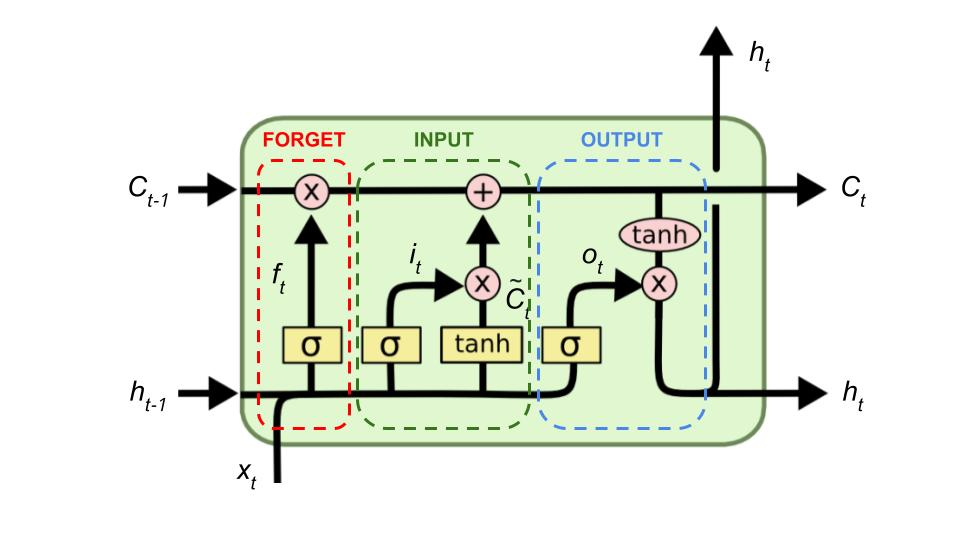
\includegraphics[width=0.5\linewidth]{figures/lstm}
  \caption{LSTM structure.}
  \label{fig:lstm}
\end{figure}

% Equations
The following sets of equations are the mathematical definition of the LSTM cell
\begin{align}
f_t &= \sigma \left( W_f h_{t-1} + U_f x_t + b_f \right)  \label{eq:lstm1} \\
i_t &= \sigma \left( W_i h_{t-1} + U_i x_t + b_i \right)  \label{eq:lstm2} \\
\tilde{C}_t &= tanh \left( W_C h_{t-1} + U_C x_t + b_C \right)  \label{eq:lstm3} \\
C_t &= f_t \cdot C_{t-1} + i_t \cdot \tilde{C}_t          \label{eq:lstm3} \\
o_t &= \sigma \left( W_o h_{t-1} + U_o x_t + b_o \right)  \label{eq:lstm4} \\
h_t &= o_t \cdot tanh \left( C_t \right)                  \label{eq:lstm5}
\end{align}
where $W$ and $b$ are the weights and biases for the different layers as in any other type of network.
The forget gate output $f_t$ is a number between 0 and 1, wherein a value of 0 means forget everything, and a value of 1, forget nothing.
In the input gate, $i_t$ defines which values to update, and $\tilde{C}_t$ comprises the candidate values that can be added into the cell state.
The cell state $C_t$ is calculated as the addition of the values not forgotten from the previous cell state $C_{t-1}$ and the new updated values $\tilde{C}_t$.
Finally, the hidden state $h_t$ is a filtered version of the cell state $C_t$, and $o_t$ decides what information is included.

% This technique is able to consider additional explanatory variables while learning across time-series \cite{calkoen_traditional_2021}.

\subsection{Optimization}
\label{sec:opt}

% Good explanation: https://distill.pub/2020/bayesian-optimization/

% BAYESIAN OPTIMIZATION USING GAUSSIAN PROCESSES
Bayesian optimization targets systems where the objective function $f$ does not have a closed form or is expensive to evaluate.
The idea of Bayesian methods is to update the current hypothesis as new information becomes available.
The process initialization uses a Gaussian process as a prior probability distribution.
In Gaussian processes, every finite collection of random variables has a multivariate normal distribution.

The prior probability represents what is originally believed before new evidence is introduced.
The routine updates a posterior probability distribution of $f$ every time a new function evaluation is reported.
This posterior model is a simpler surrogate function $\hat{f}$ approximating the objective function. 

The surrogate is easier to optimize than the objective function.
The method finds the sample that performs best on the surrogate function to evaluate it on the objective function.
An acquisition function guides the selection of the next sample from the search space.
The \textit{expected improvement} is one of the most common acquisition functions, and it indicates the region of the search space that is most likely to improve.
Overall, this method allows to reduce the number of evaluations necessary to determine the optimal parameters.

In summary, the algorithm can be itemized as follows
\begin{enumerate}
\item Place a Gaussian process prior on $f$.
\item Observe $f$ for random samples of the search space.
\item Update the $\hat{f}$ using all the available data.
\item Find the point in the search space $x_i$ that maximizes the acquisition function.
\item Get a new observation of $f$ at $x_i$.
\item Repeat 3- to 5- until convergence.
\end{enumerate}

% cite: https://mlconf.com/blog/lets-talk-bayesian-optimization/
\begin{figure}[htbp!] % or H
  \centering
  \begin{subfigure}[b]{0.49\textwidth}
    \centering
    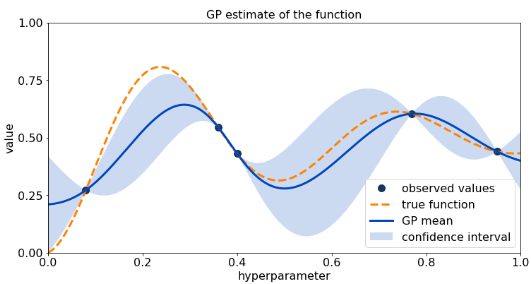
\includegraphics[width=0.85\textwidth]{figures/BO-GP-1}
    \caption{}
  \end{subfigure}
  \hfill
  \begin{subfigure}[b]{0.49\textwidth}
    \centering
    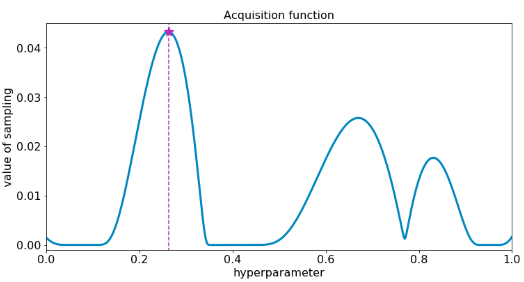
\includegraphics[width=0.85\textwidth]{figures/BO-GP-2}
    \caption{}
  \end{subfigure}
  \par
  \begin{subfigure}[b]{0.49\textwidth}
    \centering
    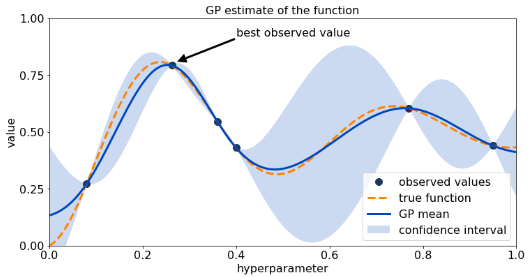
\includegraphics[width=0.85\textwidth]{figures/BO-GP-3}
    \caption{}
  \end{subfigure}
  \caption{Example of Bayesian Optimization process. Image reproduced from \cite{ravikumar_lets_2018}.}
  \label{fig:3-bo}
\end{figure}

Figure \ref{fig:3-bo} displays items 3- to 5-, where $\hat{f}$ is updated with all the available data, the process finds the point $x_i$ that maximizes the acquisition function, and, finally, $f$ is evaluated at the new observation point $x_i$. 
This work utilizes Bayesian optimization using Gaussian processes implemented through the function \textit{gp\_minimize} \cite{scikit_optimize} to optimize the different machine learning algorithms.
